\documentclass[UTF8,fontset=fandol,11pt]{ctexart}
\usepackage[a4paper,margin=24mm,headheight=15pt]{geometry}
\usepackage{amsmath,amssymb,amsthm,mathtools,bm}
\usepackage{enumitem,booktabs,longtable,array,pdfpages,fancyhdr,xcolor}
\usepackage[colorlinks=true,linkcolor=blue!45!black,urlcolor=blue!45!black]{hyperref}
\allowdisplaybreaks[2]
\setlength{\parindent}{2em}
\setlength{\parskip}{3pt}
\setlength{\emergencystretch}{3em}
\setlist{nosep,topsep=3pt}
\pagestyle{fancy}\fancyhf{}\fancyhead[L]{\small 分析学讲义习题解答}\fancyhead[R]{\small 第38--57讲}\fancyfoot[C]{\thepage}
\newcommand{\R}{\mathbb R}\newcommand{\C}{\mathbb C}\newcommand{\N}{\mathbb N}\newcommand{\Z}{\mathbb Z}\newcommand{\Q}{\mathbb Q}\newcommand{\T}{\mathbb T}
\newcommand{\dd}{\,\mathrm d}\newcommand{\eps}{\varepsilon}\newcommand{\ind}{\mathbf1}
\newcommand{\norm}[1]{\left\lVert#1\right\rVert}\newcommand{\abs}[1]{\left|#1\right|}\newcommand{\ip}[2]{\left\langle#1,#2\right\rangle}
\DeclareMathOperator{\supp}{supp}\DeclareMathOperator{\rank}{rank}\DeclareMathOperator{\Span}{Span}\DeclareMathOperator{\diag}{diag}\DeclareMathOperator{\Res}{Res}\DeclareMathOperator{\Ext}{Ext}
\newcommand{\problem}[2]{\subsection*{#1}\addcontentsline{toc}{subsection}{#1}\noindent\textbf{题干。}#2\par\smallskip\noindent\textbf{解答。}}
\newcommand{\fix}[1]{\par\noindent\textcolor{red!55!black}{\textbf{原文核对与修正。}#1}\par}
\newcommand{\skipnote}[1]{\par\noindent\textbf{依约不解的计算题。}#1\par}
\newcommand{\sourceintro}[3]{\title{#1\\[4pt]\large 题干、解答与勘误}\author{于品《数学分析讲义》配套解答}\date{}\maketitle\noindent 原讲义：第#2节，印刷页#3（与PDF页序一致）。题干按数学内容重排；完整原题页附于文末，含未解的传统计算题，供逐字核对。原文中的作业提交说明及引文不作为本项目的工作指令。\par 本文中的“正函数”均按非负函数理解。复内积约定对第一个变量线性。}
\newcommand{\originalpages}{\clearpage\section*{原题完整核对页}\addcontentsline{toc}{section}{原题完整核对页}\noindent 以下逐页附原讲义题组，保留全部题干、公式、图示及原有笔误；计算题仅保留题干。\clearpage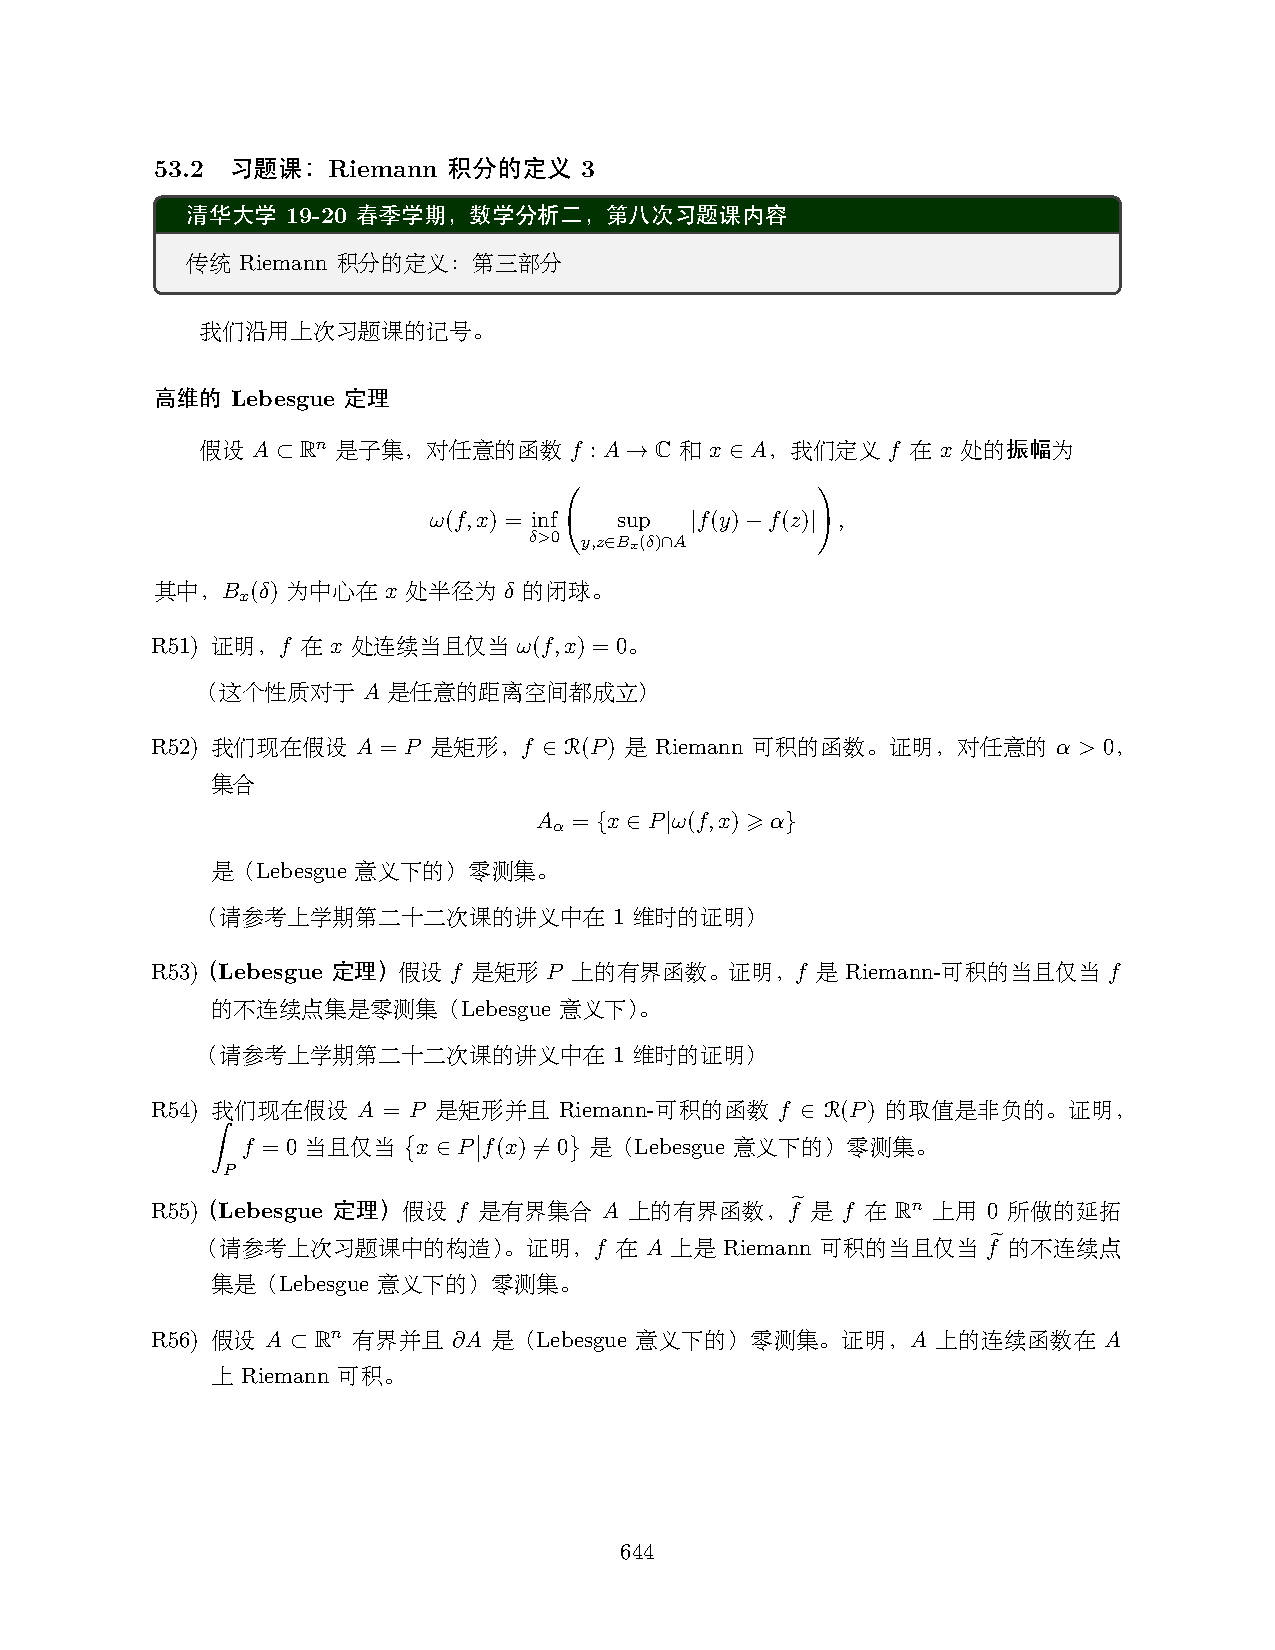
\includepdf[pages=-,pagecommand={\thispagestyle{empty}},scale=.94]{original.pdf}}

\begin{document}
\sourceintro{53.2 习题课：Riemann积分的定义3}{53.2}{644--646}
\section*{所用知识}
48.2及51.2建立的Riemann积分；第21讲的一维振幅思路，第38--45讲的零测集、完备化和测度连续性。不用把Lebesgue积分等价性作为Lebesgue判据的前提。
\section{振幅与Lebesgue判据}
对$f:A\to\C$定义$\omega(f,x)=\inf_{\delta>0}\sup_{y,z\in A\cap B(x,\delta)}|f(y)-f(z)|$。
\problem{R51}{证明$f$在$x$连续当且仅当$\omega(f,x)=0$。}
连续时在小邻域内每个值与$f(x)$之差$<\eps/2$，振幅$<\eps$。反向在振幅$<\eps$的邻域中固定$z=x$，得到连续性定义。
\problem{R52}{若$f\in R(P)$，证明每个$\alpha>0$的集合$A_\alpha=\{x:\omega(f,x)\ge\alpha\}$零测。}
选阶梯近似$|f-\varphi|\le\psi$且$\int\psi<\eps$，共同相容网格面记为$H$。若$x\notin H$，邻域内$\varphi,\psi$常值，所以$\omega(f,x)\le2\psi(x)$。故$A_\alpha\subset H\cup\{\psi\ge\alpha/2\}$；后者在各开格中为常数条件，体积至多$2\int\psi/\alpha$，面$H$零测。让$\eps\downarrow0$得到外测度零。
\problem{R53}{对矩形上有界$f$，证明Riemann可积当且仅当不连续点集为Lebesgue零测。}
必要性由R51--R52和$D_f=\bigcup_{r\ge1}A_{1/r}$。充分性先对实函数，$|f|\le M$。$A_\alpha$是闭集：若某点振幅小于$\alpha$，在足够小的邻域内其他点也有振幅小于$\alpha$。所以$A_\alpha$紧且零测，可置于总体积$<\eps$的有限开矩形并$U$中。对紧集$P\setminus U$各点选振幅$<\alpha$的邻域，有限覆盖及Lebesgue数保证足够细网格中，任何击中$P\setminus U$的格振幅$<\alpha$；其余格全部在$U$内。因此上下和差$\le\alpha m(P)+2M\eps$。令二者趋零，用Darboux判据。复函数分别对实部虚部应用；不连续点集包含各自不连续点集，反向可积后由R52得到。
\problem{R54}{非负$f\in R(P)$，证明$\int_Pf=0$当且仅当$\{f\ne0\}$零测。}
若积分零，48.2 R24说明每个连续点的值都零，所以非零点集包含于R53的零测不连续点集。反向，每个非退化小格内部均有$f=0$的点，故可选择全为零值的Riemann和；由48.2 R17其极限即积分，因而积分零。
\problem{R55}{有界$A$上的有界$f$延零为$\widetilde f$。证明$f\in R(A)$当且仅当$\widetilde f$在$\R^n$的不连续点集零测。}
取大矩形$P$使$\overline A\subset P^\circ$，则$\widetilde f$在$P$外及$\partial P$邻域均为零。全空间不连续点集与$P$内不连续点集相同，用R53及延零定义。
\problem{R56}{原文：若$A$有界且$\partial A$零测，则$A$上连续函数Riemann可积。}
\fix{漏掉函数有界条件。例如$A=(0,1)$、$f(x)=1/x$在$A$连续，边界只有两点，但不符合Riemann可积函数必须有界的定义。正确版本是“$A$上的有界连续函数”。}
在$A^\circ$上延零函数与$f$相同而连续，在$\R^n\setminus\overline A$上恒零，故不连续点只可能在$\partial A$，由R55得到结论。
\section{抽象可铺集上的积分}
\problem{R57}{若$A$为R-零测，$f:A\to\C$有界，证明可积且$\int_Af=0$。}
若$|f|\le M$，取有限矩形覆盖$A$、体积和$<\eps/M$；将$M$乘这些矩形示性函数之和作为阶梯误差上界，近似函数取零，误差积分$<\eps$。$M=0$时显然。由定义积分为零。
\problem{R58}{有界$A,B$满足$A\cap B$为R-零测，$f$定义在$A\cup B$。证明在$A,B,A\cup B$任意两个上可积即在第三个上可积，并且$\int_{A\cup B}f=\int_Af+\int_Bf$。}
已知任意两个上的可积性均使$f$在并集上有界：若已知并集则直接，若已知$A,B$则取两个界的最大值。由R57，$f\ind_{A\cap B}$的延零函数可积且积分零。恒等式
\[f\ind_{A\cup B}=f\ind_A+f\ind_B-f\ind_{A\cap B}\]
在任意共同大矩形上成立，线性性给出第三者的可积性及等式。
\problem{R59}{若$f\in R(A)$而$B\subset A$抽象可铺，证明$f|_B\in R(B)$。}
在共同大矩形上，$\widetilde f\ind_B$是两个可积函数的乘积，且为$f|_B$的延零。
\problem{R60}{若$A$抽象可铺，$f\in R(A)$，$\overline f$是在$\overline A$上的任意有界延拓，证明每个$A^\circ\subset B\subset\overline A$上的限制可积且$\int_B\overline f=\int_Af$。}
两种延零函数只在$\partial A$上可能不同。该边界为紧零测集，从而R-零测；差函数有界，R57说明其可积且积分零。
\problem{R61}{若$A$抽象可铺，证明每个$A^\circ\subset B\subset\overline A$均抽象可铺且$m(B)=m(A)$。}
在R60中取$f=1$并在闭包上也延拓为$1$。等价地，两个示性函数之差仅支撑于R-零测边界。
\problem{R62（Chasles）}{有限个抽象可铺$A_i$的两两交为R-零测，证明$f$在其并上可积当且仅当每个限制可积；并证明$\int_{\cup A_i}f=\sum_i\int_{A_i}f$。}
正向用R59。反向用R58归纳，因为$A_N\cap\bigcup_{i<N}A_i\subset\bigcup_{i<N}(A_N\cap A_i)$仍R-零测。每一步积分加性均由R58得到。
\problem{R63}{若$A$抽象可铺，$f$有界且在$A^\circ$连续，证明$f\in R(A)$。}
延零函数在$A^\circ$及闭包外连续，故不连续集包含于零测边界，使用R55。
\problem{R64}{若$A$为紧抽象可铺集，$f$连续，证明$f\in R(A)$。}
紧性给出有界性，再用R63。
\section{与Lebesgue积分的联系}
\problem{R65}{证明抽象可铺集Lebesgue可测；原题括号中还称“Borel集未必是Lebesgue可测集”。}
\fix{末句方向写反：每个Borel集都Lebesgue可测，但Lebesgue可测集未必是Borel集。}
由$A=A^\circ\cup(A\cap\partial A)$，内部为Borel集，边界是Borel零测集，故$A$属于Borel测度的完备化。也可取$B_1=A^\circ,B_2=\overline A$，二者之差零测，恰符合原题给出的夹逼定义。
\problem{R66}{若$A$抽象可铺，$f\in R(A)$，证明$f$Lebesgue可积且其Lebesgue积分等于Riemann积分。}
在$P$上取阶梯近似$|\widetilde f-\varphi_k|\le\psi_k$，并选择$\int\psi_k\le2^{-2k}$。阶梯函数在网格面上的任意有界赋值只发生于零测集，故在完备化下可测，其两种积分相同。由Chebyshev及第一Borel--Cantelli引理，除零测集外$\psi_k\to0$（例如$\sum_km(\psi_k>2^{-k})\le\sum_k2^{-k}$）。于是$\widetilde f$几乎处处为可测$\varphi_k$的极限，在完备化中可测。它有界且支撑于有限测度$P$，故可积；又$\int|\widetilde f-\varphi_k|\le\int\psi_k\to0$，所以Lebesgue积分等于$\lim\int\varphi_k$，这正是Riemann积分的定义。限制回$A$即得。
\originalpages
\end{document}
